\chapter{کاربردهای امنیتی و بانکی}
\label{chap:banking}
%=====================================================================

\section{اهمیت راهبردی بخش بانکی}

بخش بانکی به دلایل زیر یکی از اولویت‌دارترین بخش‌های اقتصادی برای پیاده‌سازی زودهنگام \lr{QKD/PQC} است:

\begin{itemize}
\item حجم بسیار بالای تراکنش‌های مالی که ارزش محرمانگی بلندمدت دارند (حساب‌های تسویه، الگوریتم‌های معاملاتی اختصاصی)؛
\item الزامات قانونی سخت‌گیرانه دربارهٔ یکپارچگی و عدم‌انکار تراکنش‌ها (که مستقیماً به امضای دیجیتال و \lr{ML-DSA} مرتبط است)؛
\item تمرکز جغرافیایی مراکز داده که پیاده‌سازی حلقه‌های \lr{QKD} کلان‌شهری با فاصلهٔ کوتاه را عملی می‌سازد؛
\item ریسک شهرت و اعتماد عمومی که هرگونه رخنهٔ امنیتی در نظام بانکی ایجاد می‌کند.
\end{itemize}

\section{تجربهٔ بین‌المللی بانک‌ها}
\label{sec:bankexperience}

نزدیک به $80\%$ از $50$ بانک بزرگ جهان اکنون به‌طور فعال در حوزهٔ فناوری کوانتومی سرمایه‌گذاری می‌کنند و این روند از فاز آزمایشی به سرمایه‌گذاری راهبردی تغییر یافته است \Cite{techinformed2025banks}. نمونه‌های برجستهٔ اجرایی عبارت‌اند از:

\begin{itemize}
\item \textbf{اولین انتقال بانکی مبتنی بر \lr{QKD} در جهان:} در سال $2004$ در وین، اتریش انجام شد \Cite{arxiv2604ipsec}.
\item \textbf{\lr{HSBC}:} در چارچوب «شبکهٔ متروی امن کوانتومی» \lr{(Quantum-Secured Metro Network, QSMN)}، پروژهٔ مشترک \lr{Toshiba} و \lr{BT Group}، ارتباط میان دفتر مرکزی \lr{Canary Wharf} در لندن و یک مرکز داده در فاصلهٔ $62$ کیلومتری را با \lr{QKD} ایمن کرده است \Cite{bankingvision2026}. این بانک هم‌چنین یک معاملهٔ شبیه‌سازی‌شدهٔ ارزی به ارزش $30$ میلیون یورو را با ترکیب \lr{QKD} و \lr{PQC} ایمن کرد، نخستین آزمایش جهانی حفاظت کوانتومی از یک پایانهٔ معاملاتی زنده \Cite{isaca2025}؛ و در پروژه‌ای جداگانه، از \lr{PQC} برای ایمن‌سازی تراکنش‌های طلای توکنیزه‌شده روی بستر \lr{Orion} استفاده کرده است.
\item \textbf{\lr{JPMorgan Chase}:} شبکهٔ \lr{«Q-CAN» (Quantum-secured Crypto-Agile Network)} این بانک، دو مرکز داده را روی فیبر مستقر با کانال \lr{VPN}\LTRfootnote{Virtual Private Network} کوانتومی-امن با ظرفیت $100$ گیگابیت بر ثانیه به یکدیگر متصل کرده است \Cite{jpmorgan2024qcan}. در آزمایشی پیشرفته‌تر با همکاری \lr{Toshiba} و \lr{Ciena}، این بانک یک کانال $800$ گیگابیت بر ثانیهٔ کوانتومی-امن را برای ایمن‌سازی شبکهٔ بلاک‌چین تولیدی \lr{Kinexys Liink} پیاده‌سازی کرد، نخستین کاربرد \lr{QKD} برای حفاظت از یک برنامهٔ بلاک‌چین حیاتی در صنعت \Cite{jpmorgan2026blockchain}.
\item \textbf{سنگاپور:} بانک مرکزی سنگاپور \lr{(Monetary Authority of Singapore, MAS)} به همراه چهار بانک بزرگ (\lr{DBS}، \lr{HSBC}، \lr{OCBC}، \lr{UOB}) و شرکت‌های فناور \lr{SpeQtral} و \lr{SPTel}، یک محیط آزمایشی \lr{(Sandbox)} \lr{QKD} مالی را روی زیرساخت ملی \lr{NQSN+} راه‌اندازی کردند و گزارش فنی نهایی آن در سال $2026$ منتشر شد \Cite{mas2026sandbox}.
\end{itemize}

شکل \ref{fig:bankadopters} خلاصه‌ای تصویری از این پنج نمونهٔ برجستهٔ بانکی را ارائه می‌دهد.

\begin{figure}[htbp]
\centering
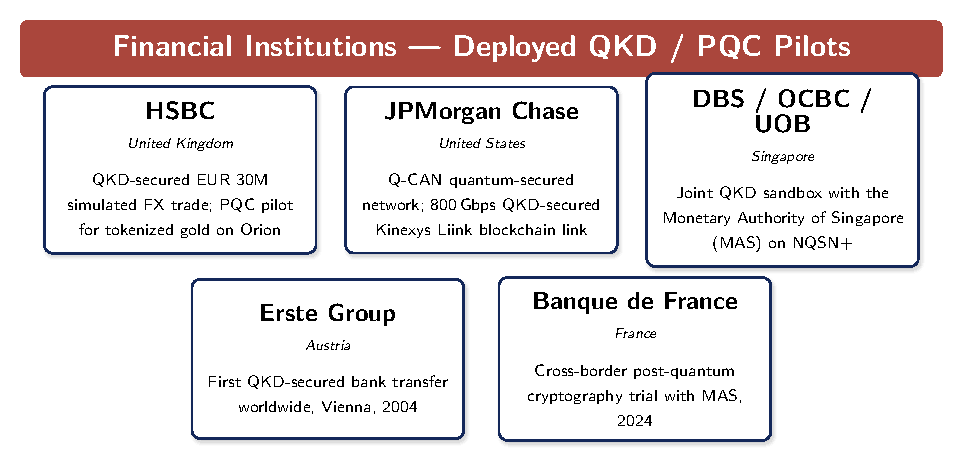
\includegraphics[width=0.98\linewidth]{figs/fig_bank_adopters.pdf}
% TODO: لوگو، نام‌های پیشنهادی فایل در figs/logos/README.txt
% \vspace{4pt}
% \includegraphics[height=1.1cm]{figs/logos/hsbc.png}\hfill
% \includegraphics[height=1.1cm]{figs/logos/jpmorgan.png}
\caption{نهادهای مالی پیشرو در پیاده‌سازی آزمایشی \lr{QKD} و \lr{PQC} \Cite{arxiv2604ipsec,jpmorgan2024qcan,jpmorgan2026blockchain,mas2026sandbox,bankingvision2026}}
\label{fig:bankadopters}
\end{figure}

\section{بحث تخصصی: امنیت گره مورد اعتماد در کاربرد بانکی}
\label{sec:bankingtrustednode}

با توجه به اینکه بسیاری از شبکه‌های \lr{QKD} کلان‌شهری، از جمله طرح پیشنهادی این سند برای تهران، برای اتصال چند مرکز داده در فاصلهٔ بیش از $100$ کیلومتر نیازمند حداقل یک گرهٔ مورد اعتماد هستند، لازم است الزامات امنیتی زیر برای هر گره به‌صورت اجباری رعایت شود:

\begin{enumerate}
\item استقرار در تأسیسات با استاندارد امنیت فیزیکی مشابه مراکز داده طبقهٔ \lr{Tier III} یا بالاتر، با کنترل دسترسی چندعاملی؛
\item ممیزی مستمر پرسنل دارای دسترسی فیزیکی (مشابه الزامات \lr{PCI-DSS}\LTRfootnote{Payment Card Industry Data Security Standard} در صنعت پرداخت)؛
\item رمزگذاری کلید در حافظهٔ گره با استفاده از ماژول‌های امنیتی سخت‌افزاری \lr{(Hardware Security Module, HSM)} سازگار با \lr{PQC}؛
\item حذف خودکار کلید از حافظهٔ گره بلافاصله پس از رمزگذاری مجدد و انتقال؛
\item در صورت امکان، استفاده از پروتکل \lr{MDI-QKD} برای گره‌های حساس، که در آن حتی گرهٔ اندازه‌گیری نیز نیازی به اعتماد کامل ندارد و آسیب‌پذیری کانال جانبی آشکارساز (نظیر حملهٔ «کوری‌سازی آشکارساز» \lr{Detector-Blinding Attack}) به‌طور بنیادین حذف می‌شود.
\end{enumerate}

این ملاحظات در فصل \ref{chap:security} (تحلیل ریسک) با جزئیات بیشتری بسط داده می‌شوند.

%=====================================================================
